\documentclass[11pt,a4paper]{report}
\usepackage[utf8]{inputenc}


\counterwithin{figure}{chapter}
\renewcommand\thefigure{\arabic{chapter} / \arabic{figure}}

\counterwithin{equation}{chapter}
\renewcommand\theequation{Equ. \arabic{equation}}

% removing of chapter titles
% from https://tex.stackexchange.com/a/121464/284352
\usepackage[pagestyles]{titlesec}
\titleformat{\chapter}[display]{\normalfont\bfseries}{}{0pt}{\Huge}
\newpagestyle{mystyle}
{\sethead[\thepage][][\chaptertitle]{}{}{\thepage}}
\pagestyle{mystyle}


\usepackage[T1]{fontenc}
\usepackage{amsmath}
\usepackage{amssymb}
\usepackage{graphicx}
%\usepackage[magyar]{babel}
\usepackage{float}
\usepackage{siunitx}
\DeclareSIUnit\decade{decade}
\DeclareSIUnit\rpm{RPM}
\sisetup{per-mode=symbol}
\usepackage{hyperref}
\usepackage{csquotes}
\usepackage[x11names]{xcolor}
\title{Teaching Your PI Controller to Behave \\ \small Technical Article(s)}
\author{Dave Wilson, Motion Products Evangelist, Texas Instruments}
\date{2013}

\hypersetup{
    pdftitle={Teaching Your PI Controller to Behave},
    pdfauthor={Dave Wilson (PDF created by HA7DN)},
    pdfsubject={Technical articles},
    pdfcreator={latex},
    pdflang=en,
    pdfkeywords={motor control, pi controller, controller tuning},
    pdfdisplaydoctitle=true,
    unicode
}
\begin{document}
    \maketitle

    \chapter{Teaching Your PI Controller to Behave (Part I)}

Richard Poley manages the training activities for our C2000 microcontrollers (MCUs), and co-teaches the TI Industrial Control Seminar series with me.  (If you have never attended one of Richard’s classes on control theory, you are really missing a spectacular treat!)  One of the stories Richard likes to tell is how the PI(D) controller was invented.  To paraphrase, a Russian-American engineer named Nicolas Minorsky was designing automatic steering systems for the US Navy in the early 1920s by observing how a helmsman steered a ship under different conditions.  According to Wikipedia.org, he noticed that the actions of the helmsman could be approximated by a simple amplification of the error signal under calm conditions, but this simple model was inadequate to describe the helmsman’s response during a steady disturbance like a stiff gale.  This finally led to the addition of an integral term to correct for continuous steady-state errors.  Later, the derivative term was added to improve controllability even further.

Continuing with the Wikipedia.org narrative, test trials of his automatic steering system based on a PI controller were first carried out on the \textit{USS New Mexico}.  After some adjustments, he was able to control the angular error to less than two degrees.  When the D term was added, the error improved to within one sixth of a degree, which was better than what most helmsmen could achieve manually!  Minorsky published his findings (also in the early 1920s), but like most famous inventions, few engineers took notice at the time.  However, we know today that his discovery launched a new era in the design of control systems!

\begin{figure}[H]
    \centering
    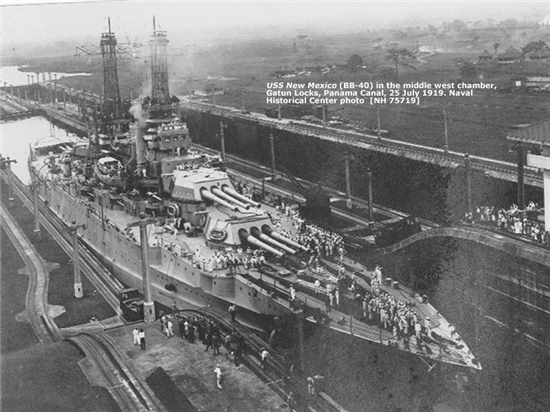
\includegraphics[width=\linewidth]{01/01_uss_new_mexico}
    \caption{\textit{U.S.S. New Mexico around the time it was retrofitted with PID control}}
    \label{fig:01ussnewmexico}
\end{figure}


    One of the questions I invariably am asked during our Industrial Control seminars is “How do you tune a PI controller?”  I typically fumble for some Bode plots or throw some simulation data up on the screen to show that the process is somewhat empirical, and very subjective to the kind of response for which you are looking.  This usually results in some disappointed stares from the audience as they realize that all I did was dodge the question instead of answering it.

After a recent seminar, I decided that I needed a better answer, so I started investigating this topic in earnest.  What I discovered changed my thinking about PI controllers!  I now believe that designing and tuning PI control loops (regardless of whether they are speed loops or current loops) is much more deterministic than I had thought!  Granted, there are still plenty of degrees of freedom depending on what kind of response you are looking for, as well as an endless litany of subtle variations on the basic PI structure itself.  But by following a few basic rules, you should be able to tune your PI loop without needing a PhD.

But first, the small print.  My analysis is limited to loads having only real poles.  If your design has prominent complex poles resulting from excessive torsional resonance between the motor and load, then the controller will have to be more sophisticated than a simple PI structure anyway to cancel the resonance effects.  But in most cases, a stiff shaft coupler should tame the torsional resonance to the point where the use of a standard PI control structure is acceptable.  Also, throughout most of this blog series I assume that the load has no viscous damping.

So, what do you think of when you hear the phrase “PI controller?”  For many, it is the conventional parallel path topology shown below.  The error signal is split into two separate paths: one which is directly amplified, and the other is amplified and then integrated.  The amplified error signal and the integrated error signal are then recombined at the output via a simple addition operation.  The integrator is included to drive the steady-state error of the system to zero, since any non-zero steady-state error will theoretically result in a boundless integrator output.  While the integrator plays a crucial role in the operation of the PI controller, it also brings a nasty set of headaches with it.  For example, let’s say that the error in your control loop is zero, which means the controlled signal is equal to the commanded signal.  Now add a small offset to the controlled signal and watch what happens.  Since the error signal is no longer zero, the integrator output will start growing …and growing …and growing in an attempt to null the error signal again.

Now remove the offset and watch what happens.  The controlled signal will eventually return to the commanded value once again, but not right away.  The integrator output is still very large, which causes the controlled signal to wildly overshoot the commanded value while the integrator output is “dumped.”  During this time, the profile of the “controlled” signal is not controlled at all, and may even result in damage to your system if not constrained.  It’s kind of like winding up a spring tightly and then suddenly releasing it.  That’s why this effect in PI controllers is called “windup.”  There are many ways to mitigate the windup effect, but most techniques involve some sort of limiting of the integrator’s output.  We will discuss this in more detail later in this series.

\begin{center}
    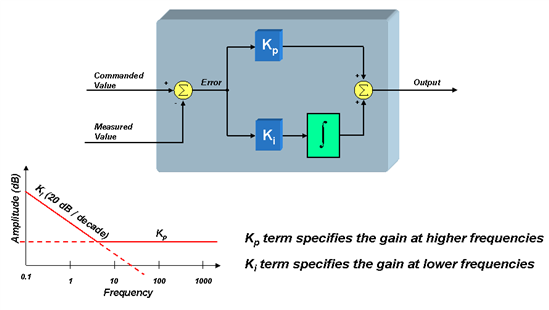
\includegraphics[width=1\linewidth]{01/02}
\end{center}

While the PI topology is fairly easy to understand, the deep dark secret is “how do you set the values for $K_p$ and $K_i$?”  This has been the subject for much debate, and it is rather difficult to intuitively understand the effect that each term has on your motor control system.  The $K_p$ term sets the high frequency gain of the control loop, as shown above.  The $K_i$ term sets the low frequency gain, and theoretically has infinite gain at DC.  The frequency which delineates the high frequencies from the low frequencies is referred to as the “zero” of the controller and corresponds to the inflection point in the frequency plot.  But we are still no closer to understanding how to set the controller’s coefficients.  So most engineers simply resort to the tried and true technique of "hit or miss."

Another popular form of the PI controller (and the one we will use for our analysis) is the “series” topology which is shown below.

\begin{center}
    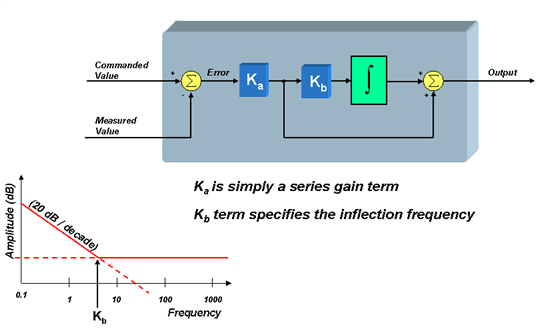
\includegraphics[width=1\linewidth]{01/03}
\end{center}

From this diagram, we can see that the relationship between the two sets of coefficients is defined as follows:

\begin{align*}
    K_a &= K_p \\
    K_b &= \frac{K_i}{K_p}
\end{align*}

But notice that in this structure, $K_a$ sets the gain for ALL frequencies, and $K_b$ directly defines the inflection point (zero) of the controller in \unit{\radian\per\second}.  Both forms are pretty much equal in terms of software implementation.  However, many engineers prefer the series form over the parallel form since $K_a$ and $K_b$ directly correlate to tangible system parameters.  It’s pretty easy to understand the effect that $K_a$ has on the controller’s performance, since it sets the gain in your open-loop transfer function.  But what is the system significance of the zero inflection point?  This is one of the discoveries I made, which I want to share with you in my next blog.  In the meantime\dots

Keep Those Motors Spinning,\\

\includegraphics[width=0.2\linewidth]{01/04_dave}
\vfill
\textit{Feb 28 2013 15:21 PM}



    \chapter{Teaching Your PI Controller to Behave (Part II)}

In my previous blog on this topic, we briefly reviewed the history of the PI controller and presented two forms that are commonly used today.  Regardless of which form you use, the frequency responses look identical.  But for our analysis, let’s focus on the \textit{series} form of the PI controller as shown below.

\begin{center}
    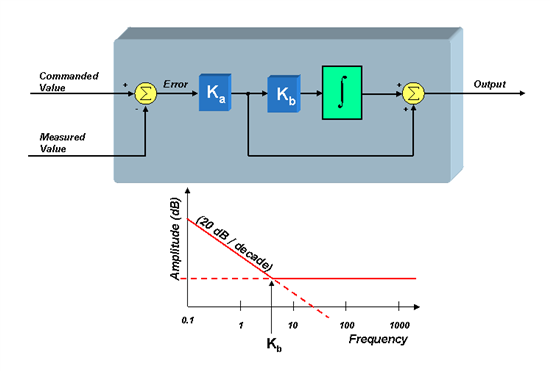
\includegraphics[width=1\linewidth]{02/01_series}
\end{center}

If you have ever done a frequency stability analysis of a control system, you probably understand why $K_a$ is so important, since it sets the gain of the PI control loop, which in turn has a pronounced effect on system stability.  But it turns out that the inflection point in the graph (the “zero” frequency) also plays a significant but perhaps more subtle role in the performance of the system.  To understand this, we will need to dive into a little math (hopefully not too much) to derive the transfer function for the PI controller, and understand how the controller’s “zero” plays a role in the overall system response.  We can define the “s-domain” transfer function from the error signal to the controller output as:
\begin{equation}
PI(s) = \frac{K_a K_b}{s} + K_a = \frac{K_aK_b \left(1+\frac{s}{K_b}\right)}{s}
\end{equation}

From this expression, we can clearly see the pole at $s = 0$, as well as the zero at $s = K_b\;(\unit{\radian\per\second})$.  So, why is the value of this zero so important?  To answer this question, let’s drop the PI controller into the heart of a current mode controller which is controlling a motor, as shown below.

\begin{center}
    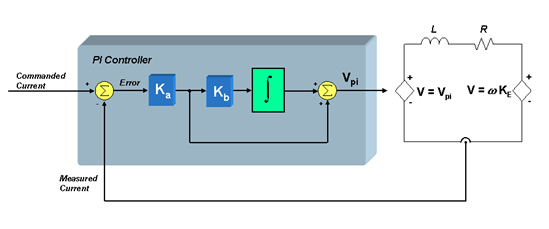
\includegraphics[width=1\linewidth]{02/02_current_mode_controller}
\end{center}

We will use a first-order approximation of the motor winding to be a simple series circuit containing a resistor, an inductor, and a back-EMF voltage source.  Assuming that the back-EMF voltage is a constant for now (since it usually changes slowly with respect to the current), we can define the small-signal transfer function from motor voltage to motor current as:
\begin{equation}
    \frac{I(s)}{V(s)} = \frac{\frac1R}{1+\frac{L}{R}s}
\end{equation}

If we also assume that the bus voltage and PWM gain scaling are included in the $K_a$ term, we can now define the “loop gain” as the product of the PI controller transfer function and the V-to-I transfer function of the RL circuit:

\begin{equation}\label{eq:3}
    G_{loop}(s) = PI(S)\cdot\frac{I(s)}{V(s)} = \left(\frac{K_aK_b \left(1+\frac{s}{K_b}\right)}{s}\right)\left(\frac{\frac1R}{1+\frac{L}{R}s}\right)
\end{equation}

To find the total system response (closed-loop gain), we must use the following expression which you probably remember from your college control systems class:

\begin{equation}\label{eq:4}
    G(s) = \frac{G_{loop}(s)}{1+G_{loop}(s)}
\end{equation}

(assuming that the feedback gain $H(s) = 1$)

Substituting \ref{eq:3} into \ref{eq:4} yields:

\begin{equation}
    G(s) = \frac{\left(\frac{K_aK_b \left(1+\frac{s}{K_b}\right)}{s}\right)\left(\frac{\frac1R}{1+\frac{L}{R}s}\right)}{1+\left(\frac{K_aK_b \left(1+\frac{s}{K_b}\right)}{s}\right)\left(\frac{\frac1R}{1+\frac{L}{R}s}\right)}
\end{equation}

I realize the expression is getting bigger instead of smaller, but don’t freak out just yet.  With a little bit of algebraic prowess, we can reduce this expression to the following:

\begin{equation}\label{eq:6}
    G(s) = \frac{\left(1+\frac{s}{K_b}\right)}{\left(\frac{L}{K_aK_b}\right)s^2 + \left(\frac{R}{K_aK_b}+\frac{1}{K_b}\right)s + 1}
\end{equation}

The denominator is a second order expression in $s$ which means there are two poles in the transfer function.  If we are not careful with how we select $K_a$ and $K_b$, we can easily end up with complex poles (Yuck!)  Depending on how close those complex poles are to the $j\omega$ axis, our system could have some really nasty resonant peaks.  So let’s assume right away that we want to select $K_a$ and $K_b$ in such a way as to avoid complex poles.  In other words, can we put the denominator in factored form so that it looks like this:

\begin{equation}\label{eq:7}
    \left(\frac{L}{K_aK_b}\right)s^2 + \left(\frac{R}{K_aK_b}+\frac{1}{K_b}\right)s + 1 = \left(1+Cs\right)\left(1+Ds\right)
\end{equation}

where $C$ and $D$ are real numbers.

If we multiply out the expression on the right side of the equation, and compare the results with the left side of the equation, we see that in order to obtain real poles, the following conditions must be satisfied:

\begin{equation}\label{eq:8}
    \frac{L}{K_aK_b} = C\cdot D
\end{equation}

and,
\begin{equation}\label{eq:9}
    \frac{R}{K_aK_b} + \frac{1}{K_b} = C + D
\end{equation}

As a first attempt to solve \ref{eq:8} and \ref{eq:9}, let’s simply equate the terms on both sides of \ref{eq:9}. In other words,

\begin{align*}
    \frac{R}{K_aK_b} &= C \\
    \frac{1}{K_b} &= D \tag{Equ. 10}\label{eq:10}
\end{align*}

The reason I recommended these substitutions will now become clear.  If we replace the denominator of \ref{eq:6} with its factored equivalent expression as shown in \ref{eq:7}, and then make the substitutions recommended in \ref{eq:10}, we get the following:

\begin{equation}\label{eq:11}
    G(s) = \frac{\left(1+\frac{s}{K_b}\right)}{\left(1+\frac{R}{K_aK_b}s\right)\left(1+\frac{s}{K_b}\right)}
\end{equation}

Notice anything interesting about this expression?  It turns out that the $D$ substitution results in a pole which cancels out the zero in the closed-loop gain expression!  By choosing $C$ and $D$ correctly, we not only end up with real poles, but we can create a closed-loop system response that has only ONE real pole and NO zeros!  No peaky frequency responses or resonant conditions!  Just a beautiful single-pole low-pass roll off response!

But wait…there’s more!  (At this point I feel like an announcer for a cheap infomercial!)  By substituting the expressions for $C$ and $D$ recommended in equation 10 back into equation 8, we get the following equality:

\begin{equation}\label{eq:12}
    K_b = \frac{R}{L}
\end{equation}

Recall that $K_b$ is the frequency at which the controller zero occurs.  So in order to get the response described in \ref{eq:11}, all we have to do is to set $K_b$ (the controller zero frequency) to be equal to the pole of the plant it is controlling!

So, now that we know how to set $K_b$, what about $K_a$?  Let’s rewrite the closed-loop system response $G(s)$, making all of the substitutions we have discussed up to now, and see what we get:

\begin{equation}\label{eq:13}
    G(s) = \frac{1}{\frac{L}{K_a}s + 1} \Rightarrow K_a= L\cdot Bandwidth \;(\unit{\radian\per\second})
\end{equation}

So we see that $K_a$ directly sets the bandwidth of the control system which is scaled by the motor’s inductance.  It turns out that numerically, $K_a$ equals the inductive impedance at whatever the bandwidth cutoff frequency is.

In summary, what have we learned?  Even if you didn’t follow all the math, there are some simple rules you can use to help you design your PI controller for your current loop:

1.  $K_b$ sets the zero of the PI controller.  When controlling a plant parameter with only one real pole in its transfer function (e.g., the current in a motor), $K_b$ should be set to the value of this pole.  Doing so will result in pole/zero cancellation, and create a closed-loop response that also only has a single real pole.  If the PI controller is part of a larger control loop, $K_b$ is not visible to the outside world since it is only used for pole-zero cancellation within the PI control loop itself.

2.  $K_a$ sets the BANDWIDTH of the closed-loop system response.  As seen by \ref{eq:13}, the higher $K_a$ is, the higher the current loop bandwidth will be.  We will discuss how to select an appropriate bandwidth in a later blog.

<Whew!>  I think I blew out enough brain cells for one blog.  I realize that this got a little “mathy,” but hopefully you could follow along with my equations.  More importantly, I hope you understand what these equations are trying to tell you about how to design your PI current control loop.  In my next blog, I want to discuss how to design a cascaded PI velocity loop which contains a PI current controller within it.  In the meantime\dots

Keep Those Motors Spinning,\\

\includegraphics[width=0.2\linewidth]{01/04_dave}
\vfill
\textit{Mar 04 2013 15:01 PM}
    \chapter{Teaching Your PI Controller to Behave (Part III)}\label{ch:3}

In my last blog, I explained how to calculate the P and I coefficients (actually the $K_a$ and $K_b$ coefficients in a series structure) for a current loop PI controller for a motor.  We saw that Kb could be used to eliminate the zero in the closed-loop system response, resulting in a system having only one real pole (i.e., well behaved and stable).  $K_a$ sets the bandwidth of the closed-loop system response.

Today, let’s back out and take a look at a speed control loop which contains two PI controllers; one to control the motor’s current, and another to control the motor’s speed.  From the figure below, notice that the output of the velocity PI controller is connected as the input reference signal for the PI current controller.  This makes sense when you think about it.  If the velocity is too low, we want to increase the motor’s current to produce more torque to speed it up.  Conversely if the motor is going too fast, we want to decrease the motor’s torque (or even drive it negative) to slow the motor down.  Together, these two PI controllers form a cascaded control loop.  By “cascaded,” I mean a control system that consists of an outer loop with one or more inner loops.  In my last blog, we saw that setting the coefficients for the PI current controller is a fairly deterministic process.  Can designing the speed PI controller be just as simple?  Do the coefficient values perform the same system functions they did with the current controller?

It turns out that closing the speed loop is a little more complicated than closing the current loop.  To properly design the speed loop, we need to know more system parameters than we did for the current loop.  This can be seen in the figure below which shows all of the components that comprise a typical cascaded speed control loop.


\begin{center}
    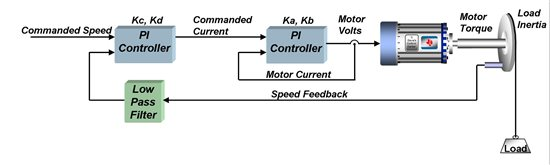
\includegraphics[width=1\linewidth]{03/01}
\end{center}

Notice that in our system, the speed feedback signal is filtered.  Unless you have an analog tachometer mounted to your motor shaft, you are probably synthesizing the speed signal by measuring other system parameters.  Even if you are using an incremental encoder on the motor shaft, you will need to synthesize velocity by measuring position.  For this reason, the speed signal often needs to be filtered before it is usable by the control system.  For our purposes, let’s just assume that we are using a single-pole low pass filter of the form:

\begin{equation}\label{eq:3_1}
    Vel_{filter}(s) = \frac{1}{\tau s+1}
\end{equation}

where $\tau$ is the time constant of the velocity filter.

Assuming we design the current loop as discussed in my previous blog, its closed-loop transfer function is:

\begin{equation}\label{eq:3_2}
    G_{current}(s) = \frac{1}{\frac{L}{K_a}s+1}
\end{equation}

where $K_a$ is the error gain term in the current regulator’s PI structure.  Recall that $K_b$ is not visible to the speed loop since it is used internally to the current loop to achieve pole-zero cancellation in its closed-loop transfer function.

I hate to do this to you again, but we are going to have to wade through a little bit more math to understand how to set the two coefficients for the speed PI controller.  To avoid confusing the coefficients of the speed controller with those of the current controller, we will call the speed controller’s coefficients $K_c$ and $K_d$ as shown in the figure above.  In the series form of the PI controller, $K_c$ will be the error gain term ($K_c = K_p$), and $K_d$ is the integrator gain term ($K_d = K_i/K_p$).  So let’s use the same equation I did in my last blog for the current controller to define the transfer function for the speed PI controller:

\begin{equation}\label{eq:3_3}
    PI_{speed}(s) = \frac{K_cK_d}{s}+K_c = \frac{K_cK_d\left(1+\frac{s}{K_d}\right)}{s}
\end{equation}

The transfer function from motor current to motor torque will vary as a function of what type of motor you are using.  Assuming we are using a Permanent Magnet Synchronous Motor under Field Oriented Control, the transfer function between q-axis current and motor torque is:

\begin{equation}\label{eq:3_4}
    Mtr(s) = \frac{3}{2}\frac{P}{2}\lambda_r = \frac{3}{4}P \lambda _r
\end{equation}
where $P = \text{the number of rotor poles}$ and $\lambda_r = \text{the rotor flux}$ (which is also equal to the back-EMF constant ($K_e$) in SI units)
\\

For reference sake, an AC Induction motor has a little bit different transfer function between q-axis current and motor torque:

\begin{equation*}
    Mtr(s) = \frac{3}{4}P \frac{}{L_m^2}{L_r}I_d
\end{equation*}

where
\begin{itemize}
    \item $P = \text{the number of stator poles}$
    \item $L_m$ is the magnetizing inductance
    \item $L_r$ is the rotor inductance
    \item $I_d$ is the component of current that is lined up with the rotor flux
\end{itemize}

But for now, let’s do the analysis using a Permanent Magnet Synchronous Motor \ref{eq:3_4}.  Moving on to the load, we see that the transfer function from motor torque to load speed (in \unit{\radian\per\second}) is:

\begin{equation}\label{eq:3_5}
    Load(s) = \frac{\omega(s)}{T(s)} = \frac{1}{Js+k_\nu}=\frac{1}{k_\nu\left(\frac{J}{k_\nu}s+1\right)}
\end{equation}
where
\begin{itemize}
    \item $J$ equals the inertia of the motor plus the load
    \item $k_\nu$ is the viscous damping term
\end{itemize}

Normally, the viscous damping factor is denoted by $k_d$, but since we have already used $k_d$ to represent one of the velocity PI coefficients, we will use $k_\nu$ to avoid confusion.  Finally, if we multiply \ref{eq:3_1} through \ref{eq:3_5} together, we achieve the composite open-loop transfer function:

\begin{equation}\label{eq:3_6}
    GH(s) = \underbrace{\left(\frac{K_cK_d\left(1+\frac{s}{K_d}\right)}{s}\right)}_{\text{Velocity PI}}
    \underbrace{\left(\frac{1}{\frac{L}{K_a}s+1}\right)}_{\text{Current Loop}}
    \underbrace{\left(\frac{3}{4}P\lambda_r\right)}_{\text{Motor}}
    \underbrace{\left(\frac{1}{k_\nu\left(\frac{J}{k_\nu}s+1\right)}\right)}_{\text{Load}}
    \underbrace{\left(\frac{1}{\tau s + 1}\right)}_{\text{Filter}}
\end{equation}

In order to untangle this mess we will make some assumptions and combine some terms.  Let’s start by assuming that the viscous damping term ($k_\nu$) is zero.  Later in this blog series we will revisit the subject of viscous damping to see what effect it has on our system.

\begin{equation}\label{eq:3_7}
    GH(s) = \underbrace{\left(\frac{K_cK_d\left(1+\frac{s}{K_d}\right)}{s}\right)}_{\text{Velocity PI}}
    \underbrace{\left(\frac{1}{\frac{L}{K_a}s+1}\right)}_{\text{Current Loop}}
    \underbrace{\left(\frac{3}{4}P\lambda_r\right)}_{\text{Motor}}
    \underbrace{\left(\frac{1}{Js}\right)}_{\text{Load}}
    \underbrace{\left(\frac{1}{\tau s + 1}\right)}_{\text{Filter}}
\end{equation}

Finally, let’s combine all the motor and load parameters into a single constant $K$:

\begin{equation}\label{eq:3_8}
    K = \frac{3P\lambda_r}{4J}
\end{equation}

Simplifying, we get:

\begin{equation}\label{eq:3_9}
    GH(s) = \frac{KK_cK_d\left(1+\frac{s}{K_d}\right)}{s^2 \left(1+\frac{L}{K_a}s\right)\left(\frac{1}{1+\tau s}\right)}
\end{equation}

From inspection of \ref{eq:3_9}, we can determine the following characteristics of the speed controller’s open-loop transfer function:
\begin{enumerate}
\item Two poles at $s = 0$, resulting in an attenuation rate at low frequencies of \qty{40}{\dB\per\decade} of frequency.
\item Two additional poles at $s = K_a/L$ (the current controller’s pole), and $s = 1/\tau$ (the velocity filter pole).
\item One zero at $s = K_d$
\end{enumerate}

For stable operation, the unity gain frequency should be higher than the zero at $s = K_d$, and lower than the two poles at $s=K_a/L$ and $s = 1/\tau$.  Other than that, there is an infinite number of combinations of $K_c$ and $K_d$ which could yield acceptable system responses, depending on whether you want higher bandwidth or better stability.  At this point, you are probably saying, “Yeah, tell me something I DON’T know!”  Well, what if I told you there was a way to take the guesswork out of the process by defining a single parameter which is proportional to system stability and inversely proportional to bandwidth, which can be used to set both $K_c$ and $K_d$ automatically?  In my next blog, I will introduce a parameter which can do just that.  In the meantime\dots \\

Keep Those Motors Spinning,\\

\includegraphics[width=0.2\linewidth]{01/04_dave}
\vfill
\textit{Mar 09 2013 14:59 PM}
    \chapter{Teaching Your PI Controller to Behave (Part IV)}

At the end of my last blog, we discussed the possibility of creating a single parameter that could automatically tune the PI coefficients for a velocity loop used in a motor speed control system.  To develop such a parameter, let’s review the open-loop transfer function for the entire velocity loop:

\begin{equation}\label{eq:4_1}
    GH(s) = \frac{KK_cK_d\left(1+\frac{s}{K_d}\right)}{s^2\left(1+\frac{L}{K_a}s\right)\left(1+\tau s\right)}
\end{equation}
where
\begin{itemize}
    \item $K$ is a coefficient that contains several terms related to the motor and load
    \item $K_c$ and $K_d$ are the PI coefficients for the velocity loop
    \item $L$ is the motor inductance
    \item $K_a$ is one of the PI coefficients for the current loop
    \item $\tau$ is the time constant of the velocity feedback filter
    \item $s$ is the Laplace frequency variable
\end{itemize}

Assuming that the zero \unit{\dB} frequency occurs somewhere between the zero at $s = K_d$ and the two nonzero poles in the denominator of the expression, we should end up with a Bode plot that looks something like this:


\begin{center}
    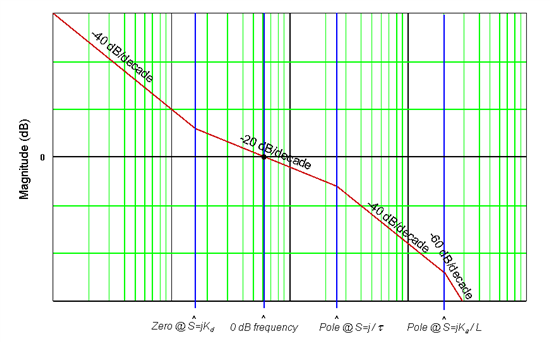
\includegraphics[width=1\linewidth]{04/01_bode}
\end{center}

The reason the shape of this curve is so important is because the phase shift at the \qty{0}{\dB} frequency determines the stability of the system.  In general, in order to get a phase shift at \qty{0}{\dB} that leads to good stability, the magnitude response should cross \qty{0}{\dB} at a rate no steeper than \qty{-20}{\dB\per\decade}.

As you can see from \ref{eq:4_1}, we must solve for three unknowns ($K_a$, $K_c$, and $K_d$) which are affected by multiple system parameters.  But instead of wading through pages and pages of esoteric equations, it’s time to make another simplification.  Let’s assume that there is only \textit{one} pole higher than the zero-dB frequency instead of two.  This assumption could mean that you don’t have a velocity filter in your system, OR that the velocity filter’s pole is \textit{way} higher than the current controller’s pole, OR that the current controller’s pole is \textit{way} higher than the velocity filter’s pole.  For most systems, it is plausible to assume the latter scenario.  So if we eliminate the effect of the current controller pole, we can rewrite the velocity open-loop transfer function as shown below:

\begin{equation}\label{eq:4_2}
    GH(s) = \frac{KK_cK_d\left(1+\frac{s}{K_d}\right)}{s^2 \left(1+\tau s\right)}
\end{equation}

For now, let’s assume that the delta in frequency between the pole $1/\tau$ and the zero $K_d$ is fixed.  In order to achieve maximum phase margin (phase shift + \qty{180}{\degree1}), the unity gain frequency should occur exactly half way in-between these two frequencies on a \underline{logarithmic} scale.  Translating from \unit{\dB} to a normal gain scale, this means the following is true:

\begin{equation}\label{eq:4_3}
    \omega_{unity\_gain} = \delta \cdot K_d
\end{equation}

and,
\begin{equation}\label{eq:4_4}
    \frac{1}{\tau} = \delta \cdot \omega_{unity\_gain}
\end{equation}

Combining \ref{eq:4_3} and \ref{eq:4_4} we can establish that:
\begin{equation} \label{eq:4_5}
    \frac{1}{\tau} = \delta^2 \cdot K_d
\end{equation}

Solving for $K_d$,
Combining \ref{eq:4_3} and \ref{eq:4_4} we can establish that:
\begin{equation}\label{eq:4_6}
    K_d = \frac{1}{\delta ^ 2 \tau}
\end{equation}

Where “$\delta$”we will define as the "damping factor."  If $\delta$ is increased, it forces the zero corner frequency ($K_d$) and the velocity filter pole ($1/\tau$) to be further apart.  And the further apart they are, the phase margin is allowed to peak to a higher value in-between these frequencies.  This improves stability but unfortunately reduces system bandwidth.  If $\delta = 1$, then the zero corner frequency and the velocity filter pole are right on top of each other, resulting in pole/zero cancellation.  In this case the system will be unstable.  Theoretically, any value of $\delta > 1$ is stable since phase margin > 0.  However, values of $\delta$ close to 1 are usually not practical as they result in severely underdamped performance.

I will talk more about $\delta$ later.  But for now, let’s turn our attention towards finding $K_c$.  From \ref{eq:4_3} we see that the open-loop transfer function of the speed loop will be unity gain at a frequency equal to the zero frequency ($K_d$) multiplied by $\delta$.  In other words,

\begin{equation}\label{eq:4_7}
    \left|\frac{KK_cK_d \left(1+\frac{s}{K_d}\right)}{s^2 \left(1+\frac{s}{\delta^2 K_d}\right)}\right|_{s=j\delta K_d} = 1
\end{equation}

By performing the indicated substitution for “$s$” in \ref{eq:4_7}, we obtain:

\begin{equation}\label{eq:4_8}
    \left|\frac{KK_cK_d \left(1+j\delta\right)}{-\delta^2 K_d^2 \left(1+\frac{j}{\delta}\right)}\right| = 1
\end{equation}

We can see that the expression within the magnitude brackets is a scalar term multiplied by a vector term.  So we can pull the absolute value of the scalar term out of the brackets, resulting in the following expression:

\begin{equation}\label{eq:4_9}
    \frac{KK_cK_d}{\delta^2 K_d^2}\left|\frac{\left(1+j\delta\right)}{\left(1+\frac{j}{\delta}\right)}\right| = 1
\end{equation}

It can be shown that the magnitude of the vector inside of the magnitude brackets is simply equal to $\delta$.  Performing this substitution and simplifying leads to the following equality:

\begin{equation}\label{eq:4_10}
    \frac{K}{\delta}\frac{K_c}{K_d} = 1
\end{equation}

Finally, we can solve for $K_c$:
\begin{equation}\label{eq:4_11}
    K_c = \frac{\delta K_d}{K} = \frac{1}{\delta K \tau}
\end{equation}

At this point, let’s step back and try to see the forest for the trees.  We have just designed a cascaded velocity controller for a motor which contains two separate PI controllers: one for the inner current loop and one for the outer velocity loop.  In order to get pole/zero cancellation in the current loop, we chose $K_b$ as follows:

\begin{equation} \label{eq:4_12}
    K_b = \frac{R}{L}
\end{equation}

Next, we select a value for the damping factor ($\delta$) which allows us to precisely quantify the tradeoff between velocity loop stability and bandwidth.  Then it’s a simple matter to calculate $K_d$ and $K_c$:

\begin{equation}\label{eq:4_6_other}
    K_d = \frac{1}{\delta^2 \tau}
    \tag{was Equ. 6}
\end{equation}

\begin{equation}\label{eq:4_11_other}
    K_c = \frac{\delta K_d}{K} = \frac{1}{\delta K \tau}
    \tag{was Equ. 11}
\end{equation}

All that remains is the selection of $K_a$ (the current controller bandwidth), which I will address in a later blog.  The benefit of this design approach is that instead of trying to empirically tune four PI coefficients which have seemingly little correlation to system performance, all you need to do is select what damping factor you want for the velocity loop.

In my next blog, let’s take a harder look at the damping factor and how it affects the performance of the velocity loop.  Until then\dots


Keep Those Motors Spinning,\\

\includegraphics[width=0.2\linewidth]{01/04_dave}
\vfill
\textit{Mar 14 2013 13:58 PM}
    \chapter{Teaching Your PI Controller to Behave (Part V)}
So far in this series, we have discussed how to distill the design of a cascaded velocity controller from a bunch of  seemingly uncorrelated PI coefficients down to a single system parameter; the \textit{damping factor} ($\delta$).  The damping factor represents the tradeoff between system stability and system bandwidth in a single parameter.  But how do you choose an appropriate damping factor value for your design, and what does it mean in terms of your system’s transient response?

To help answer these questions, let’s take a look at Figure \ref{fig:05_01}, which illustrates the \textit{open-loop} magnitude and phase response for a speed control system.  Note that all frequencies are scaled to the value of the velocity filter pole.  Assuming that the current controller's pole is very high with respect to this pole, the \textit{shape} of the curves won’t change, regardless of the velocity pole value.  In Figure \ref{fig:05_01}, the damping factor is swept from \num{70} to \num{1.5} in 8 discrete steps to show how it affects system response.  A $\delta$ value of \num{1.0} corresponds to the condition where the open-loop magnitude response has unity gain at the same frequency as the velocity filter's pole.  This scenario results in the velocity filter pole exactly cancelling out the zero which is creating all that nice phase lead we need to stabilize our system.  So we see that a $\delta$ value of \num{1.0} yields a system with zero phase margin, which of course is unstable.

\begin{figure}[H]
    \centering
    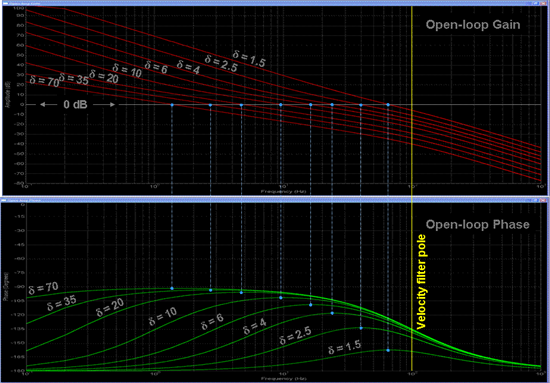
\includegraphics[width=1\linewidth]{05/01}
    \caption{Velocity Controller Open Loop Magnitude and Phase Response as a Function of $\delta$.}
    \label{fig:05_01}
\end{figure}

One of the goals of the damping factor is to achieve maximum stability for a given bandwidth.  This is confirmed in the plots above, which show that the phase margin always peaks to its maximum value at the unity gain frequency.  As the damping factor is increased, you eventually reach a point of diminishing returns for phase margin improvement as the signal phase shift approaches \qty{-90}{\degree}.  However, the \textit{gain} margin continues to improve as the damping factor is increased.

Figure \ref{fig:05_02} illustrates the \textit{closed-loop} magnitude response of the velocity loop with respect to the velocity filter pole as $\delta$ is swept from \num{70} to \num{1.5}.

\begin{figure}[H]
    \centering
    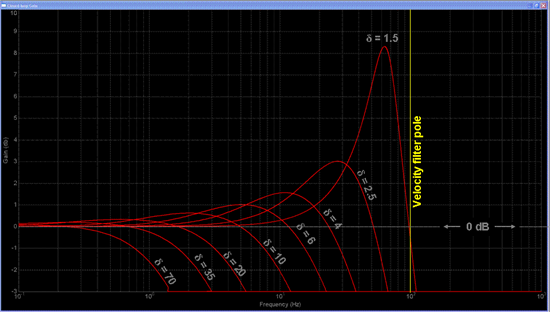
\includegraphics[width=1\linewidth]{05/02}
    \caption{Velocity Controller Closed Loop Bandwidth as a Function of $\delta$.}
    \label{fig:05_02}
\end{figure}

From figure \ref{fig:05_02} you can see how decreasing the damping factor increases the bandwidth of the velocity loop.  In fact, decreasing the damping factor from \num{70} to \num{1.5} increases the bandwidth by almost two orders of magnitude.  But as the damping factor approaches unity, the complex poles in the velocity loop approach the $j\omega$ axis, resulting in pronounced peaking of the gain response.  This peaking effect is usually undesirable, as it results in excessive underdamped ringing of the step response.  You can better see this in figure \ref{fig:05_03}, which shows the normalized step response of the system for various values of damping factor.  Values below 2 are usually unacceptable due to the large amount of overshoot they produce.  At the other end of the scale, values much above 35 produce extremely long rise and settling times.  Your design target window will usually be somewhere in-between these two values.

\begin{figure}[H]
    \centering
    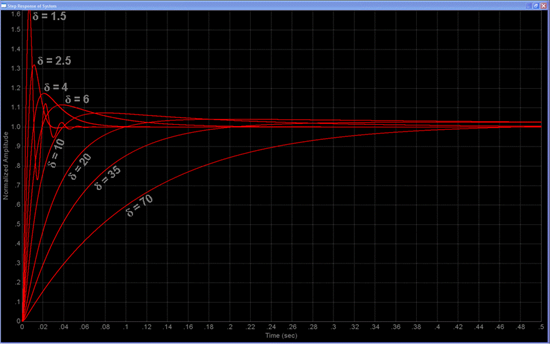
\includegraphics[width=1\linewidth]{05/03}
    \caption{Step Response of Velocity Controller as a Function of $\delta$.}
    \label{fig:05_03}
\end{figure}

What happens if you pick a damping factor based on a desired \textit{shape} for your step response, but the response \textit{time} is too long?  Well, assuming you have the design flexibility to do so, your best recourse might be to increase the velocity filter pole.  In figures \ref{fig:05_01} and \ref{fig:05_02}, all frequencies are scaled to this pole value, which means that if you change it, all other frequencies will change proportionally.  So if you double the value of the velocity filter pole in figures \ref{fig:05_01} and \ref{fig:05_02}, you will half the time axis in figure \ref{fig:05_03}.

But what if you \textit{don’t} have this flexibility?  Unfortunately, you will be forced to choose between response time and overshoot.  In other words, you can solve one problem or the other, but not both at the same time.  It’s kind of like a water balloon.  You can squeeze it down in one spot, but it will pop up somewhere else.  I know\dots it’s not fair.  But that’s the way life is sometimes.

So far we have discussed how to set three of the four PI coefficients in a velocity control loop.  But there is still one left\dots $K_a$.  Recall that $K_a$ sets the bandwidth of the current controller.  In many respects, $K_a$ is the hardest one to set since its effect on system performance is more subjective than the other three.  In my next blog, let’s take a closer look at $K_a$, its impact on system performance, and hopefully gain some insight into how to set it correctly.  In the meantime\dots

Keep Those Motors Spinning,\\

\includegraphics[width=0.2\linewidth]{01/04_dave}
\vfill
\textit{Mar 23 2013 11:13 AM}
    \chapter{Teaching Your PI Controller to Behave (Part VI)}\label{ch:6}

I am writing this particular blog installment while lying by a swimming pool in a resort on the Riviera Maya.  There are lots of beautiful distractions which are competing for my attention, including my gorgeous 20 month old granddaughter who is playing at my feet.  So I have to disclaim any liability related to the quality of this particular blog!

So far in this series we have discussed how to set the coefficients for the PI controllers in a cascaded speed control loop.  We saw that $K_b$ is used for pole-zero cancellation within the current loop.  $K_c$ and Kd are indexed to the velocity feedback filter’s time constant, and are calculated by first selecting a suitable damping factor which is related to the responsiveness and damping of the system.  We also saw that $K_a$ sets the current controller’s bandwidth.  But what should that bandwidth be?

It turns out that we have two competing effects vying for control of where we set $K_a$.  On the bottom end of the frequency range, we have the velocity feedback filter pole with some really nice tan lines that wants to push the current controller pole to higher frequencies so as to not interfere with our nice tuning procedure.  But we can only go so high before we start running into other problems.  Let’s take a look at both ends of the frequency spectrum in an effort to understand these issues, and hopefully gain some insight into how to judiciously set $K_a$.  But first, let’s rewrite the open-loop transfer function of the velocity loop to once again include the current controller’s transfer function:

\begin{equation}\label{eq:6_1}
    gH(s) = \frac{K K_cK_d \left(1+\frac{s}{K_d}\right)}{s^2 \left(1+\frac{L}{K_a}s\right)\left(1+\tau s\right)}
\end{equation}

where
\begin{itemize}
    \item $K$ is a coefficient that contains several terms related to the motor and load
    \item $K_c$ and $K_d$ are the PI coefficients for the velocity loop
    \item $L$ is the motor inductance
    \item $K_a$ is one of the PI coefficients for the current loop
    \item $t$ is the time constant of the velocity feedback filter
    \item $s$ is the Laplace frequency variable
\end{itemize}

Our tuning procedure assumes that the current controller’s closed-loop gain is always unity, which implies it has infinite bandwidth.  But in reality, as long as the current controller’s bandwidth is at least 10x higher than the velocity loop unity gain frequency, our tuning procedure is still pretty good at predicting the system response.  If this condition isn’t satisfied, the current controller pole starts interfering with the velocity loop phase margin, resulting in a more underdamped response than our tuning procedure would otherwise indicate.

Figure \ref{fig:06_01} shows an example case to illustrate this point.  The {\color{SpringGreen4}green} curve represents what the tuning procedure predicts the normalized step response should be for a system with a damping factor of \num{2.5}.  The {\color{red}red} curve shows what happens when the current controller’s bandwidth is reduced to equal the velocity filter’s bandwidth.  The system is still stable, but the damping is much less than predicted from our tuning procedure.  At this point, we have two options\dots either increase the damping factor (and consequently lower the frequency response of the velocity loop), or increase the current loop bandwidth by increasing $K_a$.  The {\color{Cyan4}cyan} curve shows the first option where we increase the damping factor just enough to bring the overshoot down to the predicted value.  Unfortunately this increases the step response transient time as well.  The {\color{Gold2}yellow} curve shows the latter option where we put the damping factor back to \num{2.5}, and increase the current controller’s pole to be 10x higher than the velocity loop unity gain frequency.  As you can see, the actual response more closely resembles the predicted value.  The higher the current controller’s bandwidth is, the closer the response will resemble the predicted response.

\begin{figure}[H]
    \centering
    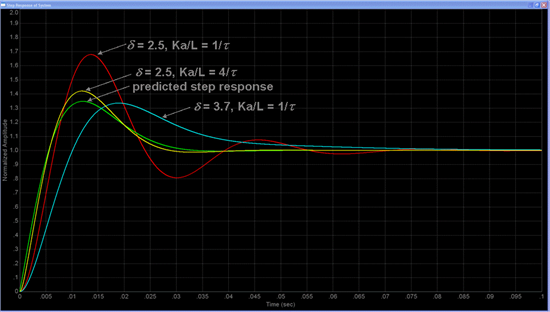
\includegraphics[width=1\linewidth]{06/01}
    \caption{Step Response of a System with Variable Damping and Pole Placement}
    \label{fig:06_01}
\end{figure}

So from this exercise, we might conclude that the best strategy is to set the current controller bandwidth to be as high as possible.  But is this really the best course of action?  As my dear ol’ grandma used to say, “Never use a 1 \unit{\giga\Hz} op-amp when a \qty{1}{\mega\Hz} op-amp will do the job.”  (Well, she never actually said it in those exact words, but you get the point).  Usually high bandwidth in \textit{any} system results in unruly and obnoxious behavior, and should only be used if absolutely necessary.  In this case, high current loop bandwidth often results in undue stress on your motor, since high frequency \textit{current} transients and noise translate into high frequency \textit{torque} transients and noise.  This can even manifest itself as \textit{audible} noise!  But there is also another limit on your current loop bandwidth:  the \textit{sampling frequency}.

Take a look at Figure \ref{fig:06_02} which shows a digital Field Oriented Control (FOC) based Variable Frequency Drive (VFD).  To simplify the discussion, we will assume that the entire control loop is clocked by a common sampling signal, although in real-world applications we often choose to sample the velocity loop at a much lower frequency than the current loop to save processor bandwidth.

\begin{figure}[H]
    \centering
    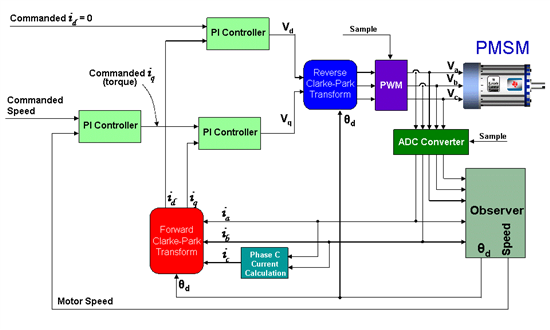
\includegraphics[width=1\linewidth]{06/02}
    \caption{Digital Field Oriented Control System for a PMSM.}
    \label{fig:06_02}
\end{figure}

In an analog system, any change in the motor feedback signals immediately starts having an effect on the output control voltages.  But with the digital control system of Figure \ref{fig:06_02}, the motor signals are sampled via the ADC at the beginning of the PWM cycle, the control calculations are performed, and the resulting control voltages are deposited into double-buffered PWM registers.  These values sit unused in the PWM registers until they are clocked to the PWM output at the start of the next PWM cycle.  From a system modeling perspective, this looks like a sample-and-hold function with a sampling frequency equal to the PWM update rate frequency.  The fixed time delay from the sample-and-hold shows up as a lagging phase angle which gets progressively worse at higher frequencies.  Figure \ref{fig:06_03} shows a normalized frequency plot of the phase delay for a sample-and-hold function, where the sampling frequency is assumed to be 1.  As you can see, the phase delay reaches down into frequencies much lower than the sampling frequency.  For example, at one decade below the sampling frequency, the S\&H is still affecting a phase shift of \qty{-18}{\degree}.

\begin{figure}[H]
    \centering
    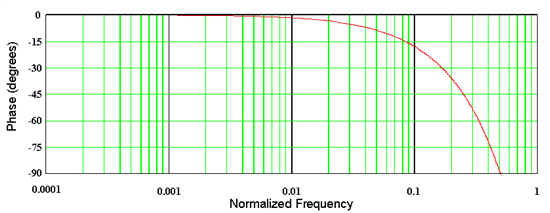
\includegraphics[width=1\linewidth]{06/03}
    \caption{Phase Lag Plot for a Sample-and-Hold, $F_s = 1$}
    \label{fig:06_03}
\end{figure}

Since the current controller processes higher bandwidth signals than the velocity loop, it is usually the current loop that suffers most by the S\&H effect of the PWM module.  Since the PWM S\&H is in series with the signal path for the current loop, its magnitude and phase contributions add directly to the open-loop response for the current controller.  If we rewrite the equation for the open-loop response of the current controller (assuming $K_b = R/L$), we end up with the following function:

\begin{equation} \label{eq:6_2}
    GH_c(s) = PI(s) \cdot \frac{I(s)}{V(s)} = \left(\frac{K_a}L\right)\left(\frac1s\right)
\end{equation}

This is simply an integrator function with gain of $K_a/L$.  Unity gain will obviously occur when $s = K_a/L$.  The single pole at $s = 0$ implies that the unity gain frequency will have a \qty{90}{\degree} phase shift, which also implies a \qty{90}{\degree} phase margin.  However, for a digital control system, you must add the phase lag shown in Figure \ref{fig:06_03}.  To do this, calculate for the following frequency ratio:

\begin{equation} \label{eq:6_3}
    \frac{K_a T_s}{2\pi L}\,\text{where $T_s$ is the sampling period}
\end{equation}

Then use Figure \ref{fig:06_03} to determine how much phase lag you must subtract off of your phase margin.  For example, if $K_aT_s/(2\pi L) = 0.1$, then you must subtract off \qty{18}{\degree} from your phase margin, leaving you with a comfortable \qty{72}{\degree}.  In most designs you probably want to keep $Ka/(2\pi L)$ at least an order of magnitude below the sampling frequency.  So using this assumption as well as the constraints from the velocity loop tuning procedure, we can now write a general “rule of thumb” expression for the range of $K_a$:

\begin{equation}\label{eq:6_4}
    \frac{10L}{\delta \tau} < K_a < \frac{\pi L}{5 T_s}
\end{equation}
where:
\begin{itemize}
    \item $L$ is the motor inductance
    \item $\tau$ is the time constant of the velocity filter
    \item $\delta$ is the damping factor
    \item $T_s$ is the sampling period
\end{itemize}


In most designs this still leaves a fairly broad range for the value of $K_a$.  In my experience, I have found that erring on the side of the current bandwidth being too low is usually better than being too high.  Snappy waveforms look nice on an oscilloscope, but your application may not need (or want) all that bandwidth.

Up until now, we have only dealt with “small signal” conditions (i.e., linear operation with no saturation effects).  But in the real world, step transient responses almost always saturate the system’s voltage or current levels, which tend to lengthen the response times.  When this happens, you can increase the PI gains all you want, but it won’t speed up the response.  In fact, it will usually just make the overshoot worse, since the integrator is acting on a gained-up error signal, which it will just have to dump eventually.  So how do we deal with this problem?  Are we doomed to simply using low integrator gains?  It turns out that there is another solution which doesn’t involve changing your integrator gains, which I will discuss in my next blog.  Until then\dots\\


Keep Those Motors Spinning,\\

\includegraphics[width=0.2\linewidth]{01/04_dave}
\vfill
\textit{Apr 04 2013 23:24 PM}
    \chapter{Teaching Your PI Controller to Behave (Part VII)}

So far we have discussed the PI tuning problem in the context of a linear system.  This is because under steady-state conditions when the system transients settle out, you will probably be operating in the linear region, and \textit{that’s} when your feedback loop will either oscillate or not.  Therefore, performing a small-signal (linear) analysis will tell you how stable your system will be when it is not saturated.  But in most real-life scenarios, the system \textit{will} saturate because of limits on your voltage and/or current, especially under large transient conditions.  This saturation effect can play some real mind games with your PI controller; especially the integrator.  Since the maximum torque your motor can produce is determined by your current limit, the acceleration of the system is also limited.  But the integrator in the PI speed controller doesn’t know this, and it thinks it can make the motor speed up even faster by increasing its output.  This increased integrator output can’t help the situation since the system is already saturated.  All it does is create a very large output that will cause the system to overshoot when it \textit{does} come out of saturation.  For this reason, most PI integrators employ techniques to keep them from needlessly integrating while the system is saturated.

One technique which is commonly used is \textit{integrator clamping}, which establishes limits for the maximum and minimum values that the integrator output can have.  An example of this is illustrated in Figure \ref{fig:07_01}.  The most common scenario is to set the clamp values to be equal to the PI output limit values.  However, there is nothing that says that the integrator limits must \textit{equal} the PI output limits, and many designs use different clamp values based on the specific application.  As you might expect, the tighter you set the clamp limits, the less windup you will have to deal with when the system finally does come out of saturation.

\begin{figure}[H]
    \centering
    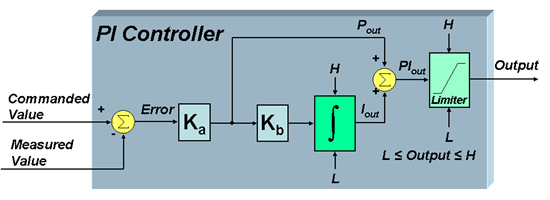
\includegraphics[width=1\linewidth]{07/01}
    \caption{PI Controller with Static Integrator Clamping}
    \label{fig:07_01}
\end{figure}

However, a more robust clamping scheme is shown in Figure \ref{fig:07_02}.  The thinking behind \textit{dynamic integrator clamping} is based on the rationale that if the system is already saturated by the P gain output, then why allow the integrator to continue integrating since it can’t help anyway.  Only during conditions where changes in the integrator output would affect changes in the PI controller output is the integrator allowed to integrate the error signal.


\begin{figure}[H]
    \centering
    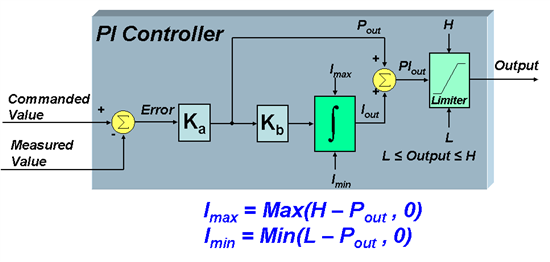
\includegraphics[width=1\linewidth]{07/02}
    \caption{PI Controller with Dynamic Integrator Clamping}
    \label{fig:07_02}
\end{figure}

The effectiveness of integrator clamping can be seen by the simulated velocity responses in Figure \ref{fig:07_03}.  The system is instantly stimulated with a commanded velocity step from zero to a target speed of \qty{1500}{\rpm}, which will obviously cause saturation.  Shown are the effects of system overshoot with \textit{no} clamping, \textit{static} clamping where the integrator clamp values equal the output clamp values, and finally \textit{dynamic} clamping.  As you can see, no integrator clamping at all is unacceptable as it results in horrendous overshoot which triggers further system saturation and oscillation.  Static integrator clamping dramatically improves the system response.  However, dynamic clamping improves performance even further, resulting in six times less overshoot than static clamping in this particular example.  An important but somewhat obvious point to remember about integrator clamping is that it only improves the overshoot response if the clamp activates.  If the commanded stimulation is small enough to keep the system in the linear mode of operation, then the overshoot you get will be determined exclusively by the damping factor.

\begin{figure}[H]
    \centering
    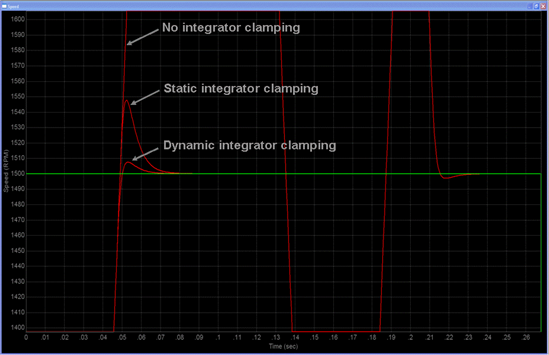
\includegraphics[width=1\linewidth]{07/03}
    \caption{Example Comparison of Integrator Clamping Techniques}
    \label{fig:07_03}
\end{figure}

Another technique that has been used to mitigate windup is \textit{integrator switching}.  With this technique, the integrator is only turned on at the \textit{end} of a commanded profile transition, or when the system output has pulled to within a specified range of the commanded input.  In the latter case, the output loading must be small (or at least somewhat predictable) in order to select a meaningful threshold for when to turn the integrator on.  But you must also be careful how and when you turn the integrator \textit{off}.  If you also reset the integrator output to zero when you switch it off, you can end up with a large and undesirable discontinuity in the output waveform if the integrator output was very large at the time.  But not resetting the output to zero can also have undesirable consequences when the integrator is turned back on.  For example, if the steady-state integrator output eventually changes polarity when it is turned back on again, the settling time will take much longer than if the integrator output had been reset.  My opinion about integrator switching is that it can be an effective technique to minimize windup, but getting good results can be tricky, and it is very much application dependent.

In my next blog, I want to double back and talk some more about PI tuning.  Now that we know how to put the puzzle together, the obvious question to ask is, “do we have all the pieces?”  Up until now, I have assumed the answer is \textit{yes}.  But there is one piece that all the other pieces fit around that we haven’t really talked a lot about, and that is \textbf{inertia}.  While this parameter is sometimes provided on a motor data sheet, it is almost never provided for the load you are driving.  Without it, you can’t accurately tune your velocity loop unless you rely heavily on trial and error.  In my next blog, I want to introduce you to TI’s new InstaSPIN-FOC algorithm, and propose a technique for how it can be used to actually \textit{measure} system inertia.  You don’t want to miss this one!  Until then\dots\\

Keep Those Motors Spinning,\\

\includegraphics[width=0.2\linewidth]{01/04_dave}
\vfill
\textit{Apr 13 2013 15:56 PM}
    \chapter{Teaching Your PI Controller to Behave (Part VIII)}

We are now on the eight part of a ten part series about teaching your PI controller to behave like you want it to.  At the heart of this discussion is a proposed tuning technique which allows you to be more proactive with the tuning process and reduce the amount of empirical guesswork at the back-end of your design process.  TI has already used this tuning technique on several motor control designs with good success!  But as with any “parameter based” design process, the results are only as good as how well you know your parameters.  In summary, for a permanent magnet synchronous machine, we need to know the following parameters to tune the PI loops:
\begin{itemize}
    \item $R_s$ (motor stator resistance)
    \item $L_s$ (motor stator inductance)
    \item $P$ (\# of motor poles)
    \item $\lambda_r$ (rotor flux)
    \item $J$ (system inertia)
\end{itemize}

If you’re lucky, the motor data sheet may have some of this information.  But in many cases you’re on your own trying to figure out what they are.  But don’t despair!  TI has just released a new sensorless Field Oriented Control algorithm called InstaSPIN-FOC which can measure most of these parameters for you automatically!  Figure \ref{fig:08_01} is a high level diagram of InstaSPIN-FOC, which shows its three distinct components:

\begin{enumerate}
    \item Motor ID:  This algorithm interrogates the motor to gather most of the parameters above.  It is usually run just once during the commissioning process for a particular motor.
    \item FAST:  This is the observer which calculates the real-time motor parameters needed for Field Oriented Control.  The neat part is that it doesn’t require a shaft angle or speed sensor to do it!  F.A.S.T. stands for Flux, Angle, Speed and Torque, which represent the main outputs of the FAST observer.  A diagram of how the FAST observer can be used in a Field Oriented Controller is shown in figure \ref{fig:08_02}.
    \item PowerWarp:  This is a special energy savings operating mode used to reduce the copper losses in AC Induction Machines, especially during light-load conditions.
\end{enumerate}
\begin{figure}[H]
    \centering
    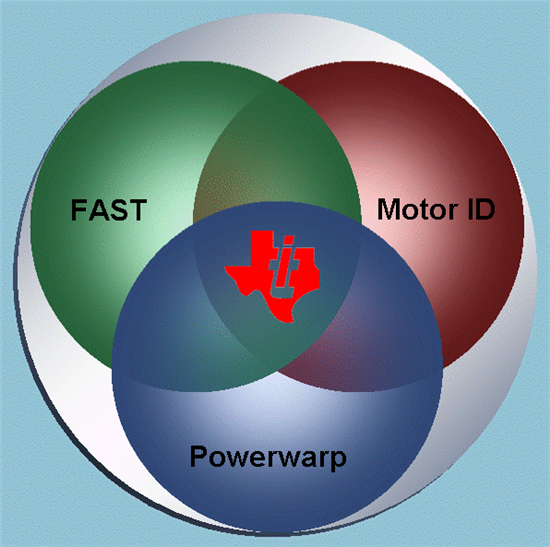
\includegraphics[width=0.8\linewidth]{08/01}
    \caption{Components of InstaSPIN-FOC}
    \label{fig:08_01}
\end{figure}

There is actually a fourth component of InstaSPIN-FOC which is part of the motor ID function, and runs in real time to provide continuous estimates of the stator resistance.  This is the parameter that typically changes the most as the motor heats up during operation.  Monitoring it in real time significantly improves the performance of the FAST observer, and also allows you to dynamically change $K_b$ in the current PI controllers to maintain pole/zero cancellation.  I have a lot more to say about this feature, as well as the other components of InstaSPIN-FOC in an upcoming blog series.

\begin{figure}[H]
    \centering
    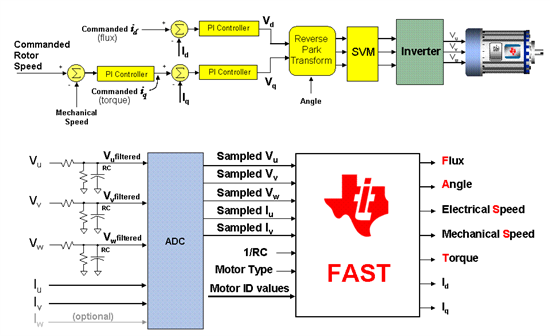
\includegraphics[width=0.8\linewidth]{08/02}
    \caption{ FAST Embedded in a Field Oriented Controller}
    \label{fig:08_02}
\end{figure}

So we see that InstaSPIN-FOC provides measurements for $R_s$, $L_s$, and the rotor flux.  Fortunately, the number of motor poles is often listed on most data sheets, or can easily be determined empirically.  This leaves only system inertia ($J$) that is unknown.  But the entire velocity loop tuning procedure hangs on whether we accurately know what this parameter is.  Even though InstaSPIN-FOC doesn’t directly measure inertia for you, the following is a proposed procedure for how to use the outputs from FAST to measure inertia:

\begin{enumerate}
\item Design the current controller by setting $K_a = L_s/\tau$, or $\pi L_s/(10T_s)$, whichever is lower.  Recall that $\tau$ equals the velocity feedback filter time constant, $L_s$ = the stator winding inductance, and $T_s$ = sampling period.  Also set $K_b = R_s/L_s$.

\item Disable the velocity loop and use only the current loop.  Set $I_d =0$, and apply a fixed value of q-axis current which is sufficient to cause the motor and load to accelerate through a good portion of the rated speed range.

\item \label{step:08_03} As the motor is ramping up to speed, periodically sample and record the values for motor mechanical speed ($\omega(n)$ in \unit{\radian\per\second}) and also the motor torque ($T_1(n)$ in \unit{\newton\meter}).  Both of these measurements are outputs from the FAST observer.  The motor torque should be pretty consistent since $I_q$ is constant, and the motor speed should monotonically increase for a well behaved load.  For example, figure \ref{fig:08_03} shows the simulated samples of the speed output from the FAST observer for a permanent magnet motor driving a fan load with fixed inertia.  The sampling frequency is \qty{200}{\milli\second} over a \qty{4}{\second} span, resulting in a total of 20 samples.
% Note: here I found the first typo in those blogposts: it said 200 mS vs 200 ms
\item Now enable the velocity loop and set the PI coefficients to very low values that will barely allow you to spin the motor up to speed.  Since we don’t know inertia yet, we can’t accurately specify the velocity loop coefficients anyway.  Don’t worry about the dynamic response of the system at this point, since we are only interested in steady state performance.

\item Command the motor to go to each of the recorded speeds from step \ref{step:08_03} by monitoring the speed output of the FAST observer.  After the system response has completely settled out for each commanded velocity, again record the torque values from FAST ($T_2(n)$ in \unit{\newton\meter}).  This torque will correspond to the static load torque apart from any acceleration artifacts.

\item We now have all the data required to solve for inertia as a function of time ($J(n)$ in \unit{\kg\m\squared}) by using the following difference equation:
\begin{equation}\label{eq:8_1}
    \hat J(n) = \frac{2 T_s \left(T_1(n-1) - T_2 (n-1)\right)}{\omega(n)-\omega(n-2)}
\end{equation}
where
\begin{itemize}
    \item $J(n)$ is the inertia at sample time "$n$" (\unit{\kg\m\squared})

    \item $T_s$ is the periodic sampling period (\unit{s})

    \item $T_1$ is the total torque consisting of static friction and acceleration torque (\unit{\newton\meter}) from the FAST observer

    \item $T_2$ is the static friction torque only (\unit{\newton\meter}) from the FAST observer

    \item $w$ is the mechanical speed measurement (\unit{\radian\per\second}) from the FAST observer
\end{itemize}
\end{enumerate}

\begin{figure}[H]
    \centering
    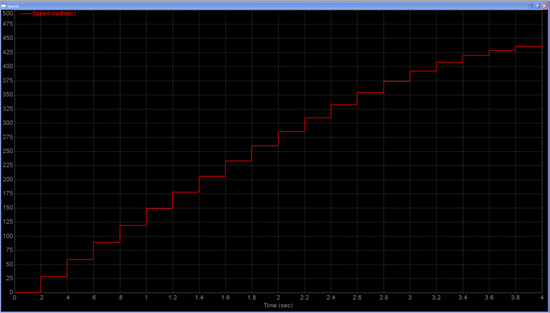
\includegraphics[width=0.8\linewidth]{08/03}
    \caption{Simulated Speed Samples of a Fan Controller with Fixed Inertia}
    \label{fig:08_03}
\end{figure}


Figure \ref{fig:08_04} shows an example inertia plot using \ref{eq:8_1} applied to the data from figure \ref{fig:08_03}.  The estimated values are plotted in red at each time step along with the actual load inertia in green.  In this particular scenario, the inertia is constant and the torque ripple is zero, making it the best condition to estimate inertia.  As you can see, the results are most accurate for the range in figure \ref{fig:08_03} where the acceleration is fairly constant.  In this case you would simply time-average those inertia estimates to come up with a single value for system inertia.  But what if you have excessive torque ripple, such as a compressor load?  In that case, you can think of the torque ripple as unwanted noise in the system.  To maximize the signal-to-noise ratio, you should set the q-axis current as high as possible to increase the ratio between the $T_1$ and $T_2$ torque readings.  It would also help to do a time average of the steady-state torque readings at each velocity point.



\begin{figure}[H]
    \centering
    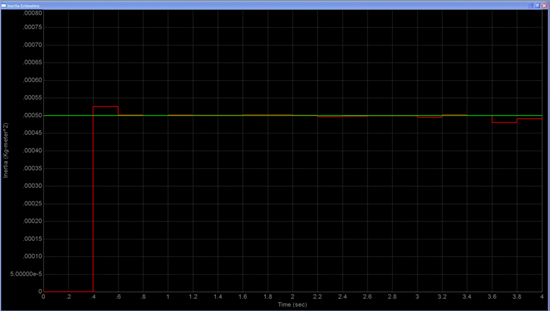
\includegraphics[width=0.8\linewidth]{08/04}
    \caption{Estimated vs. Actual Values of System Inertia as a Function of Time}
    \label{fig:08_04}
\end{figure}

For applications where inertia is a function of velocity (like a centrifuge load), this technique can provide a distinct advantage over other techniques.  Since equation \ref{eq:8_1} calculates inertia as a function of time, and you also have data for motor speed as a function of time from step \ref{step:08_03}, you can combine the two sets of data to correlate inertia as a function of speed.  Having this data in a Look Up Table in memory allows you to dynamically update the $K_c$ term in the velocity PI controller as the speed changes to optimize the response at any speed.

So far, we have discussed PI tuning in generic terms which are mostly independent of the control topology.  In my next blog, I want to focus specifically on some of the more subtle points to consider when designing PI controllers for Field Oriented Control systems.  Until then\dots

\;\\\;\\
Keep Those Motors Spinning,\\

\includegraphics[width=0.2\linewidth]{01/04_dave}
\vfill
\textit{Apr 14 2013 22:35 PM}
    \chapter{Teaching Your PI Controller to Behave (Part IX)}

At last!  Let’s take what we have learned so far and see how it applies to Field Oriented Control (FOC) systems.  Figure \ref{fig:09_01} shows a typical field oriented system incorporating TI’s new FAST sensorless observer.  Recall from my last blog that FAST stands for Flux, Angle, Speed, and Torque.  As with most speed control systems based on FOC, this diagram utilizes three PI controllers; two for controlling the quadrature components of current, and one for controlling the velocity.

\begin{figure}[H]
    \centering
    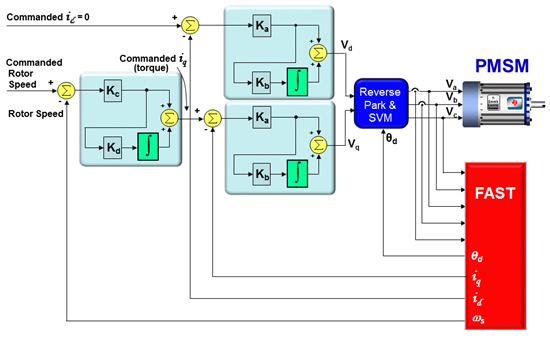
\includegraphics[width=0.8\linewidth]{09/01}
    \caption{Typical FOC Speed Control of a PMSM}
    \label{fig:09_01}
\end{figure}

The design of the velocity controller doesn’t change much in a field oriented system compared to other control algorithms.  But there are subtle differences which affect how you should design your current controllers, which are listed below.

\begin{enumerate}
    \item The motor’s equivalent RL circuit seen by the controllers (which determines how you set the PI coefficients) will vary depending on the motor type.  For BLDC and Permanent Magnet Synchronous Motors (PMSMs), $R$ is simply the stator resistance, and $L$ is the stator inductance.  As we have seen up to now, the PI coefficients are the same for the d and q current regulators.  But with AC Induction Motors (ACIMs), this is not the case.  For the d-axis, the resistance is equal to the stator resistance, just like it is with a PMSM.  But inspection of the rotor flux-based model of an AC induction motor reveals that the q-axis current controller sees an equivalent resistance equal to the stator resistance PLUS the rotor resistance.  Another difference is the inductance value you should use for both axes.  It turns out that it is not the stator inductance value, but rather the “series” inductance (or sometimes called the “leakage” inductance) which is defined as follows:

    \begin{equation}\label{eq:9_1}
        L = L_s \left(1-\frac{L_m^2}{L_sL_r}\right) = L_s \cdot \sigma
    \end{equation}
    where
    \begin{itemize}
        \item  $L$ = the equivalent series inductance
        \item  $L_s$ = the stator inductance
        \item  $L_m$ = the magnetizing inductance
        \item  $L_r$ = the rotor inductance
        \item  $\sigma$ = the “leakage factor” of the induction motor
    \end{itemize}

    Finally, it turns out that an IPM motor should be handled differently than either a PMSM or an ACIM.  The resistance value used by both the d and q axis current controllers is the stator resistance (just like any other PMSM).  The value used for inductance is the stator inductance, also similar to PMSMs.  But the stator inductance is different between the d and q axes, where $L_q$ is usually larger than $L_d$ due to the lower flux reluctance along that axis.

    In many cases these subtleties between motors won’t cause a big difference in the performance of your system, especially since you only have one pole in your current controller transfer function, and you can afford to be somewhat conservative.  But in higher performance, higher bandwidth systems, these subtleties must be considered, or you could end up with a PI current controller that is incompatible with your motor, resulting in less than optimal control.  As a first step in helping you manage all these different conditions, I have designed a \href{https://web.archive.org/web/20180101224106/http://e2e.ti.com/cfs-file/__key/telligent-evolution-components-attachments/13-852-00-00-00-66-49-89/PI-Calculator.xlsx?forcedownload=true}{spreadsheet} which can help you calculate the PI coefficients as a function of motor type for a field-oriented system.  The white cells represent fields that you must populate with data, and the grey cells will be calculated automatically based on the data you enter.  Go ahead and try it!  Just be mindful to use the correct SI units listed in each column, or you will not get the results you want.

    \item  It turns out that the control of the d-axis and q-axis currents are not independent from one another.  Within the motor, there is a natural cross coupling between the d-axis and q-axis which can be seen in the differential equations below for a PMSM:

    \begin{align}
        i_d \left(R+DL_s\right) &= V_d + \omega L_s i_q  \label{eq:9_2}\\
        i_q \left(R+DL_s\right) &= V_q - \omega \left(L_s i_d + K_e\right) \label{eq:9_3}
    \end{align}
    where
    \begin{itemize}
        \item $R$ is the stator resistance
        \item $L_s$ is the stator inductance
        \item $D$ is the differential operator
        \item $\omega$ is the electrical frequency
        \item $K_e$ = the Back EMF constant
    \end{itemize}

    From \ref{eq:9_2} we see that $V_d$ is not the only voltage term vying for control of the d-axis current.   There is also a speed dependent term which contains $i_q$ in it.  From \ref{eq:9_3}, $V_q$ is also competing with a voltage term containing $i_d$.  For both regulators, this cross-coupling effect manifests itself as an unwanted disturbance which is most prominent during transient conditions at high speeds.  To correct for this situation, feed-forward decoupling can be applied to each axis which exactly cancels these cross-coupled voltage terms.  The result is the regulator topology shown in Figure \ref{fig:09_02}.
\begin{figure}[H]
    \centering
    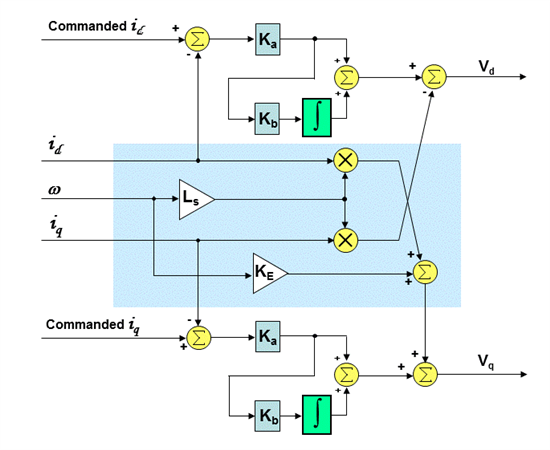
\includegraphics[width=0.8\linewidth]{09/02}
    \caption{Decoupled PI Controllers for a PMSM}
    \label{fig:09_02}
\end{figure}

    For AC Induction Motors, the correction becomes a little bit more sophisticated.  The differential equations defining AC induction motor operation are shown below:

    \begin{align}
        i_d \left(R_s+DL_s\sigma\right) &= V_d + \omega L_s \sigma i_q -\frac{L_m}{L_r}D\lambda_{rd} \label{eq:9_4}\\
        i_q \left(R_s+DL_s\sigma\right) &= V_q - \omega L_s \sigma i_d - \omega \frac{L_m}{L_r}\lambda_{rd} \label{eq:9_5}
    \end{align}
    where
    \begin{itemize}
        \item $R_s$ = the stator resistance
        \item $L_s$ = the stator inductance
        \item $\sigma$ = the leakage factor defined in \ref{eq:9_1}
        \item $D$ is the differential operator
        \item $\omega$ =  the electrical frequency
        \item $L_m$ = the magnetizing inductance
        \item $L_r$ = the rotor inductance
        \item $\lambda_{rd}$ = the d-axis rotor flux
    \end{itemize}

    Similar to the situation with a PMSM machine, we see that there are other voltages besides $V_d$ and $V_q$ vying for control of $i_d$ and $i_q$ respectively.  As a result, compensation voltages must be added to $V_d$ and $V_q$ to nullify these other voltage terms.  The compensation block used to provide correction voltages to the outputs of the $i_d$ and $i_q$ regulators is shown in Figure \ref{fig:09_03}.

    \begin{figure}[H]
        \centering
        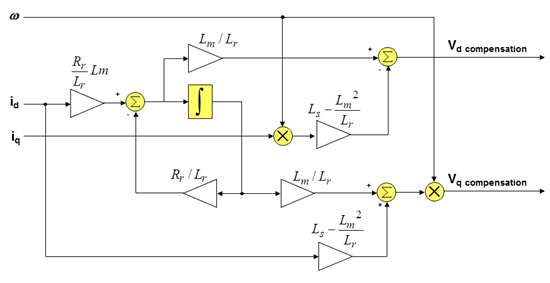
\includegraphics[width=0.8\linewidth]{09/03}
        \caption{Compensation Block used for Axis Decoupling with ACIMs.}
        \label{fig:09_03}
    \end{figure}

    As an example of the effectiveness of this technique, consider the simulation results of figure \ref{fig:09_04} which show the $i_d$ and $i_q$ waveforms for a 3 HP AC induction machine.  Without axis decoupling you can see how transient changes in $i_q$ current spill over into the d-axis.  This deviation from the commanded d-axis current will also cause an undesirable perturbation in the motor’s flux.  In the bottom graph we can see that the q-axis regulator is also ineffective at regulating $i_q$ during sudden changes in velocity.  But when the decoupling scheme of figure \ref{fig:09_03} is enabled, $i_d$ and $i_q$ currents track their respective commanded values much more precisely.


    \begin{figure}[H]
        \centering
        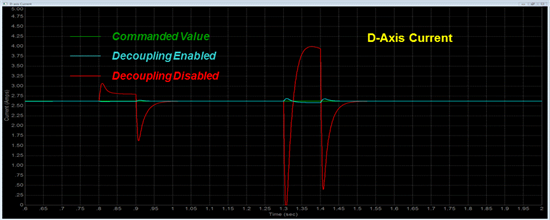
\includegraphics[width=0.8\linewidth]{09/04}
        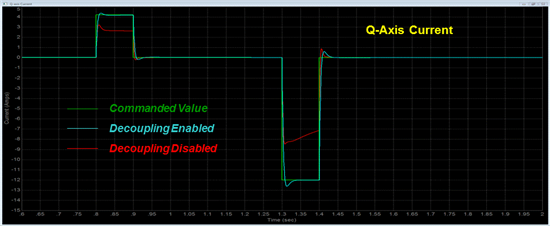
\includegraphics[width=0.8\linewidth]{09/05}
        \caption{Id and Iq Waveforms with and without Axis Decoupling.}
        \label{fig:09_04}
    \end{figure}

    A final thought about coupling compensation.  If you examine figures \ref{fig:09_02} and \ref{fig:09_03} you can see that what we are really doing is applying feed-forward signals to both the d and q regulator outputs.  The good news is that since this doesn’t add any poles to your closed-loop system, it is inherently stable.  But a word of caution\dots the feed-forward paths can inject very high frequencies from one axis into the other.  In some cases, this can excite your system with unwanted high frequency harmonics which can cause unwanted and unexpected behavior. This is especially true if you are operating the motor in field-weakened mode at high speeds.  Under these conditions you typically want to “handle with care”, or you can temporarily lose control of the motor.
\end{enumerate}

In my next and final blog entry on this topic, I would like to offer some concluding remarks regarding developing and debugging this PI tuning technique in a digital control system, as well as investigate the case where viscous damping is present.  In the meantime\dots


Keep Those Motors Spinning,\\

\includegraphics[width=0.2\linewidth]{01/04_dave}
\vfill
\textit{Apr 30 2013 17:32 PM}
\newpage
\textbf{UPDATE  July 19th, 2013}:  There have been several questions related to how I calculate the back-EMF constant ($K_e$) in my equations.  Several individuals have tried to use my \href{https://web.archive.org/web/20180101224106/http://e2e.ti.com/cfs-file/__key/telligent-evolution-components-attachments/13-852-00-00-00-66-49-89/PI-Calculator.xlsx?forcedownload=true}{spreadsheet} with their motor designs, only to obtain incorrect results which can be traced back to how $K_e$ is represented.

It turns out that the units for $K_e$ in my \href{https://web.archive.org/web/20180101224106/http://e2e.ti.com/cfs-file/__key/telligent-evolution-components-attachments/13-852-00-00-00-66-49-89/PI-Calculator.xlsx?forcedownload=true}{spreadsheet} are “volts (peak, line-to-neutral) per electrical radian per second”.  By representing $K_e$ in SI units like this, its numerical value is equivalent to the motor flux (in Webers).  Unfortunately, very few (if any) motor manufacturers represent back-EMF this way.  This means that you must convert your datasheet value for $K_e$ into the above units in order for the spreadsheet to yield correct results.  For example, Teknic Inc (as well as many other motor manufacturers) represents the back-EMF for their PMSM machines in volts (peak) per 1k RPM.  In just about every case, it is implied that this voltage is line-to-line since you usually can’t directly measure the line-to-neutral voltage.  To convert from these units to the SI units used in my spreadsheet, you must use the following multiplication factor:
\begin{equation*}
    \frac{\sqrt 3}{50 \pi P}
\end{equation*}
where P is the number of rotor poles.

The following multiplication factors can be used to convert the back-EMF units most frequently found on motor data sheets into the SI units in my spreadsheet:

\begin{tabular}{cc}
    \textbf{\underline{To convert from}} & \textbf{\underline{Multiply by}}\\
    Volts(peak, line-to-line) per electrical Hz  & $\frac{1}{2\pi\sqrt3}$ \\
    Volts(peak, line-to-line) per electrical radian/sec &  $\frac1{\sqrt 3}$\\
    Volts(peak, line-to-line) per mechanical radian/sec  & $\frac2{P\sqrt 3}$ \\
    Volts(peak, line-to-line) per kRPM & $\frac{\sqrt 3}{50\pi P}$ \\
    Volts(RMS, line-to-line) per electrical Hz & $\frac{1}{\pi \sqrt 6}$ \\
    Volts(RMS, line-to-line) per electrical radian/sec & $\sqrt{\frac{2}{3}}$ \\
    Volts(RMS, line-to-line) per mechanical radian/sec & $\frac{2}{P}\sqrt{\frac{2}{3}}$ \\
    Volts(RMS, line-to-line) per kRPM & $\frac{\sqrt 6}{50 \pi P}$ \\
\end{tabular}
    \chapter{Teaching Your PI Controller to Behave (Part X)}

Throughout this series we have discussed a practical and efficient way to tune the PI controllers in a cascaded velocity loop by simply choosing a factor that determines the desired damping of the system.  From this information, plus a rudimentary knowledge of some of the motor and load parameters, the PI coefficients for the velocity loop and the inner current loops can be calculated.  We developed this technique by first ignoring certain aspects of the control loop, such as the pole of the current controller.  But in blog \ref{ch:6} we reintroduced the current controller’s pole back into the discussion, and evaluated its impact on system performance.

Today, let’s look at the other end of the frequency spectrum.  At low frequencies, viscous damping may affect your velocity loop response times by changing the phase margin at the unity-gain frequency.  When viscous damping is present, it siphons off part of the motor’s torque to do work to move fluid.  Since viscous torque is directly proportional to the speed of the load, we can rewrite the load’s transfer function to be:

\begin{equation}\label{eq:10_1}
    \frac{\omega(s)}{T(s)} = \frac{1}{Js+k_\nu} = \frac{1}{k_\nu \left(\frac{J}{k_\nu}s+1\right)}
\end{equation}
where $k_\nu$ is the viscous damping factor.

As you can see from \ref{eq:10_1}, adding the viscous damping term moves the pole that was at $s = 0$ to $s = k_\nu/J$.  Figure \ref{fig:10_01} shows how the addition of viscous damping changes the load’s Bode plot.

\begin{figure}[H]
    \centering
    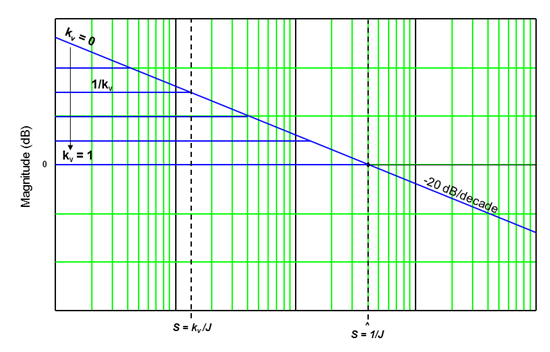
\includegraphics[width=1\linewidth]{10/01}
    \caption{Effect of Viscous Damping ($k_V$) on the Load Bode Plot}
    \label{fig:10_01}
\end{figure}

From Figure \ref{fig:10_01}, we see that as viscous damping increases from zero, low frequency gain plateaus to a value of $1/k_\nu$.  The net effect on the phase plot is to add more phase margin at lower frequencies, since the phase lag of a load with viscous damping will always be less than a load with inertia only.  As a result, stability should actually improve for non-zero values of $k_\nu$.  However, the response time may take a hit, depending on where the velocity open-loop unity-gain frequency is with respect to the pole frequencies shown in Figure \ref{fig:10_01}.  So if your system response is sluggish and the motor doesn’t seem to put out as much torque as it is rated for, you might want to investigate how much viscous damping your system has.

Before closing out this series, I want to address one more important topic.  I have seen and experienced situations myself where the PI coefficients were calculated correctly, but when they were incorporated into the code, the motor either screamed like a banshee or sat there like a lump and did nothing.  So what happened?  In many cases, it was one of the following problems:

\begin{enumerate}
    \item Forgetting to account for the sampling frequency effect on the GAIN of the integrator term.  Figure \ref{fig:10_02} shows how to implement a typical integrator for a digital PI controller.  To scale the output to match what an analog integrator would provide, we must first multiply the input signal by the sampling period “$T$”.  In order to avoid two separate multiply operations, most code examples simply lump $T$ together with the integrator gain term.  If $T$ is not accounted for, you will end up with an integrator gain that is MUCH higher than you anticipated.
    \begin{figure}[H]
        \centering
        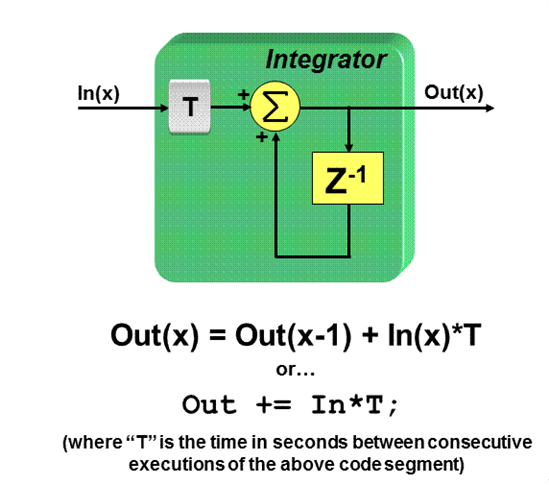
\includegraphics[width=1\linewidth]{10/02}
        \caption{Typical Implementation of a Digital Integrator}
        \label{fig:10_02}
    \end{figure}

    \item So far we have assumed there are no limitations on the number format itself.  If you are using a floating-point processor, then you don’t have to worry about the fractional component of your PI terms.  But most motor control applications are implemented on fixed-point machines for cost reasons.  The good news is that TI has developed a linkable library that is in the ROM of most of our C2000 processors which solves this problem for you.  It is called the “IQ Math” library which stands for “Integer Quotient”.  This allows you to handle floating point values with ease on a fixed-point machine without suffering from the performance hit you typically get with a full-blown floating-point package.  IQ math creates a new variable type in your code which is designated by a “Q” followed by a number.  For example, let’s say you have a 32 bit variable which is typed as a “Q24” variable type.  This means that any variable of this type is assumed to have a 24-bit fractional component, and an 8-bit integer part.  But what occasionally happens is that someone copies TI example code into their design without realizing that our coefficients are represented in IQ format.  For example, if you calculate your I-gain to be \num{10000} (\$00002710 in Q0 format), but you didn’t realize that the TI code assumes the variable is in Q24 format, you will end up with an integrator gain of \num{0.596E-3} instead of \num{10000}.  Obviously, a big difference!  If you make the same mistake for all of the PI coefficients, the motor will most likely just sit there and do nothing since all the gains are way too low.  So, a word to the wise; make sure you know what numerical format your coefficients are represented by.

    \item In some cases, the PI coefficients for an AC Induction Motor drive are calculated correctly and the motor runs just fine\dots until the motor speed exceeds its rated value, at which point the controller response becomes underdamped.  The reason for this can be found back in blog \ref{ch:3} of this series.  The motor transfer function between q-axis current and electromagnetic torque for an AC induction motor is repeated below.
    \begin{equation}
        Mtr(s) = \frac34 P \frac{L_m^2}{L_r}I_d
    \end{equation}

    For speeds up to the rated speed, $I_d$ usually stays constant.  But to achieve speeds beyond the rated speed, you need to reduce the flux in the machine by lowering the value of $I_d$.  You can probably see where I’m going with this.  When you reduce $I_d$, you reduce the gain of the entire velocity loop gain.  If it is reduced too much, you can end up moving the unity-gain frequency to a lower value where the effect of the two poles at $s=0$ have more effect on reducing the phase margin.  To keep the system response from changing, the $K_c$ (or $K_p$) term in the speed PI controller can be increased in direct proportion to the reduction in $I_d$.

    \item Finally, the scaling of the PI coefficients throughout this series has been done assuming we want to represent real system values throughout the signal chain.  For example, the output of the velocity PI controller equals the actual input reference current in amps for the current controller.  The output of the current controller equals the actual voltage applied to the motor winding.  But in many designs, the PI controller outputs are normalized to “Per Unit” (PU) scaling where a value of 1 represents the maximum value possible, and a value of -1 represents the minimum value possible.  For example, a current regulator’s output might be scaled in such a way that 1 corresponds to 100\% PWM, and -1 corresponds to 0\% PWM.  The advantage of this approach is that you can quickly adapt your code to different systems by simply changing your per unit scaling values.  To convert from real-value scaling to PU scaling for $K_a$, $K_b$, $K_c$, and $K_d$ (including the sampling period for the integrators), use the following formulae:

    \begin{equation}
        K_{a\_scaled} = K_a \frac{I_{scale}}{V_{scale}}
    \end{equation}
    where
    \begin{itemize}
        \item $I_{scale}$ is the actual current value corresponding \num{1.0}
        \item $V_{scale}$ is the actual voltage value corresponding to \num{1.0}
    \end{itemize}

    \begin{equation}
        K_{b\_scaled} = K_b T_i
    \end{equation}
    where
    \begin{itemize}
        \item $T_i$ corresponds to the sampling period of the current loop.
    \end{itemize}

    \begin{equation}
        K_{c\_scaled} = K_c \frac{Vel_{scale}}{I_{scale}}\frac{2}{P}
    \end{equation}
    where
    \begin{itemize}
        \item $Vel_{scale}$ = the actual velocity value in \unit{\radian\per\sec} corresponding to \num{1.0}
        \item $I_{scale}$ is the actual current value corresponding \num{1.0}
        \item $P$ = the number of rotor poles on the motor
    \end{itemize}

    \begin{equation}
        K_{d\_scaled} = K_d T_v
    \end{equation}
    where
    \begin{itemize}
        \item $T_v$ corresponds to the sampling period of the velocity loop.
    \end{itemize}

    The PU scaling for traditional parallel PI structures is:
    \begin{align}
        K_{p\_scaled} &= K_{c\_scaled} \\
        K_{i\_scaled} &= K_c K_d \frac{Vel_{scale}}{I_{scale}}\frac{2}{P}T_v
    \end{align}
    where
    \begin{itemize}
        \item $Vel_{scale}$ = the actual velocity value in \unit{\radian\per\sec} corresponding to \num{1.0}
        \item $I_{scale}$ is the actual current value corresponding \num{1.0}
        \item $P$ = the number of rotor poles on the motor
        \item $T_v$ corresponds to the sampling period of the velocity loop.
    \end{itemize}
\end{enumerate}

\textit{\textbf{Note from HA7DN, 2026-04-03:} I am not sure if the VisSim software mentioned here is available today, the supplied link redirects to \url{https://altair.com/embed/}, where a free trial is available, but I have not tried it.}

To assist you with the design of your FOC based speed controller, I have created a VisSim simulation (\href{https://web.archive.org/web/20130813082852/http://e2e.ti.com/group/motor/m/simulations/665001.aspx}{FOC.vsm}) which accepts inputs from an Excel spreadsheet (\href{https://web.archive.org/web/20130813082852/http://e2e.ti.com/group/motor/m/simulations/665002.aspx}{Motor.xlsx}).  If you open the spreadsheet, you can see the parameters for several different motor/load examples as well as the PI controller coefficients which are automatically calculated.  You can also add your own motor and load parameters in the spreadsheet if you want.  To create a \href{https://web.archive.org/web/20130813082852/http://e2e.ti.com/group/motor/m/simulations/665003.aspx}{text output file} which is required by the VisSim simulation, you must perform a “Save As” option, and in the “Save as Type” field, select “CSV (Comma delimited) (*.csv).”  Assuming that this file is in the same folder as "FOC.vsm", you can then open "FOC.vsm" and simply click the run icon on the toolbar at the top of the page to run the simulation.  You can see the speed response (as well as plots of other system variables) by scrolling over to the right side of the simulation window.  The simulation creates a step change in the commanded velocity at $t=0$ which saturates the system, and another step change at $t=\qty{0.5}{\s}$ which doesn’t saturate the system, allowing you to evaluate the system response under both conditions.  If you would like to evaluate another motor /load example, simply double-click on the Motor/Load Selector Block in the bottom-left corner of the simulation window and choose a different option, as shown below.

\begin{figure}[H]
    \centering
    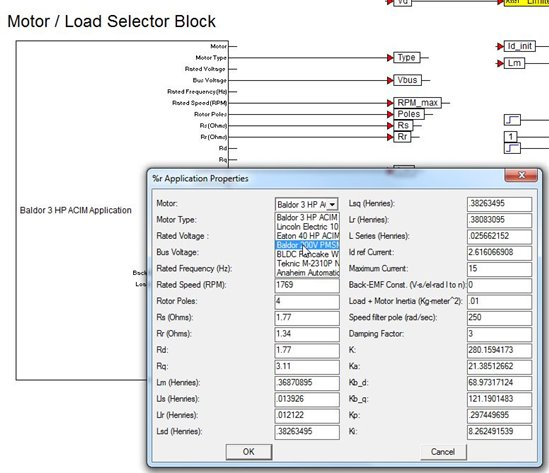
\includegraphics[width=1\linewidth]{10/03}
    \caption{Motor/Load Selector Block in the FOC.vsm Simulation File}
    \label{fig:10_03}
\end{figure}

If you would like to take this simulation out for a test drive, but you don’t have VisSim installed on your machine, simply follow the instructions below:

\begin{enumerate}
    \item Go to Visual Solutions’ \href{https://web.archive.org/web/20130813082852/http://www.vissim.com/}{website}.

    \item In the top right of the browser window, click on “Create account”

    \item After you create an account, click on the “Downloads” tab, and select “VisSim Software”.

    \item Click on the first link on the top of the page that says “VisSim -- Core simulator + UML State Charts + Analyze”

    \item Run the installer program.  This will install the free 60 day trial version of VisSim.
\end{enumerate}

Congratulations\dots we made it!  Thanks for investing your time with me as we have looked at different ways to make your PI control loop behave.  I hope you learned some neat tricks that can help you “stay in tune” with your motor control design.

By the way, if you have suggestions for other motor control topics you would like for me to address in a future blog, I would love to hear from you.  :-)  And of course\dots

Keep Those Motors Spinning,\\

\includegraphics[width=0.2\linewidth]{01/04_dave}\\
\vfill
\textit{May 15 2013 17:13 PM}\\
\url{www.ti.com/motorblog}

    \chapter*{Notes by HA7DN, editor of this PDF}

    I found one of these articles on the interwebs on 2025 March 31th as a PDF on TI's website (\url{https://www.ti.com/lit/pdf/ssztcg3}). Sadly, it looks like only the first two are available this way (second part at \url{http://www.ti.com/lit/pdf/ssztcg3}).

    I came upon the 2025 reddit post \textit{Articles by Dave Wilson on Motor Control} on \textbf{r/Motors} by user \textbf{u/suhas\_patlolla} (\url{https://www.reddit.com/r/Motors/comments/1iiu62b/articles_by_dave_wilson_on_motor_control/}), where user \textbf{u/PippoCavallo} collected the archive.org links for the articles.

    The original post:
    \begin{displayquote}[\textbf{u/suhas\_patlolla}]
        Hello, recently I was going through the youtube video where wilson teaches about old motors new tricks and in that video I have came through his blogs about "Teaching the PI controllers to behave" a 10 part series of blogs and other is "The 10 commandments of Digital Control" which is again a 10 parts.

        I can't find them any where even though the link which says ti.com/motorblogs which is not working now and I could find 2 parts but I want all others so that it will be helpful for me.

        So, if any of you guys know where to get them all or if you have them can please share me.

        I think 2014 guys will have them :)
    \end{displayquote}

    The response:
    \begin{displayquote}[\textbf{u/PippoCavallo}]
        Same of you, I was looking for them after watching the rec of the seminar. In such cases you can try to use Wayback Machine. So beautiful tool that makes me grateful many times. Enjoy!

        \url{https://web.archive.org/web/20131113220619/http://e2e.ti.com/blogs_/b/motordrivecontrol/archive/2013/02/28/teaching-your-pi-controller-to-behave-part-i.aspx}

        \url{https://web.archive.org/web/20131113212704/http://e2e.ti.com/blogs_/b/motordrivecontrol/archive/2013/03/04/teaching-your-pi-controller-to-behave-part-ii.aspx}

        \url{https://web.archive.org/web/20131113205503/http://e2e.ti.com/blogs_/b/motordrivecontrol/archive/2013/03/09/teaching-you-pi-controller-to-behave-part-iii.aspx}

        \url{https://web.archive.org/web/20131113220631/http://e2e.ti.com/blogs_/b/motordrivecontrol/archive/2013/03/14/teaching-your-pi-controller-to-behave-part-iv.aspx}

        \url{https://web.archive.org/web/20131113214729/http://e2e.ti.com/blogs_/b/motordrivecontrol/archive/2013/03/23/teaching-your-pi-controller-to-behave-part-v.aspx}

        \url{https://web.archive.org/web/20131113221525/http://e2e.ti.com/blogs_/b/motordrivecontrol/archive/2013/04/04/teaching-your-pi-controller-to-behave-part-vi.aspx}

        \url{https://web.archive.org/web/20130813082822/http://e2e.ti.com/blogs_/b/motordrivecontrol/archive/2013/04/13/teaching-your-pi-controller-to-behave-part-vii.aspx}

        \url{https://web.archive.org/web/20130813082828/http://e2e.ti.com/blogs_/b/motordrivecontrol/archive/2013/04/14/teaching-your-pi-controller-to-behave-part-viii.aspx}

        \url{https://web.archive.org/web/20130813082842/http://e2e.ti.com/blogs_/b/motordrivecontrol/archive/2013/04/30/teaching-your-pi-controller-to-behave-part-ix.aspx}

        \url{https://web.archive.org/web/20130813082852/http://e2e.ti.com/blogs_/b/motordrivecontrol/archive/2013/05/15/teaching-your-pi-controller-to-behave-part-x.aspx}

        EDIT: this is the spreadsheet referred to in the <Part IX>: \url{https://web.archive.org/web/20180101224106/http://e2e.ti.com/cfs-file/__key/telligent-evolution-components-attachments/13-852-00-00-00-66-49-89/PI-Calculator.xlsx?forcedownload=true}
    \end{displayquote}

    There was one added note:
    \begin{displayquote}[\textbf{u/PlethoraProliferator}]
         there is also a video of a shorted topic still alive at ti: \url{https://www.ti.com/video/3881562077001}
    \end{displayquote}

    Thanks \textbf{Dave Wilson} for the articles and \textbf{u/PippoCavallo} for finding all the archive.org links!

    All I did was trasnscribing the original texts to \LaTeX. Any typo you may encounter is most likely attributed to me.

    HA7DN 2026

    \chapter*{Contact}

    This PDF along with it's \LaTeX\; sources is available at \url{https://github.com/Sasszem/Teaching-Your-PI-Controller-to-Behave-by-Dave-Wilson-}. You can contact me (HA7DN) via github. If you have spotted an error / mistake in my transcription, you can submit an issue or even better a pull request.
\end{document}